\chapter{Introducci\'on} % (fold)
\label{cha:introduccion}
%\addcontentsline{toc}{chapter}{Introducción}
Hoy en día el manejo de información en la sociedad juega un papel importante en el desarrollo de las actividades que la conforman. Millones de personas en el mundo tienen la facilidad de acceder a un dispositivo electrónico que les permite manipular esta información o almacenarla para posteriormente darle un uso específico. La información que circula en dispositivos electrónicos es mayor a la memoria disponible que ofrecen estos, a medida que el volumen de información aumenta, también lo hace la demanda para los servicios de almacenamiento en línea. Un gran incremento en el uso de estos servicios implica tener más infraestructura y personal para que los sistemas de almacenamiento tengan más capacidad y puedan cubrir la demanda que se presenta en el mercado. Si bien el almacenamiento logró dar buenos resultados al cliente en sus primeras etapas, ahora la preocupación por el incremento de infraestructura para seguir dando esos resultados se ha incrementado considerablemente. ~\cite{Bellare} ~\cite{Keelveedhi}

Una de las principales razones por la que está sucediendo es que muchos usuarios almacenan un mismo archivo un claro ejemplo es que n usuarios pueden subir la misma canción, por lo tanto esta se encuentra almacenada en las n cuentas de la nube, esto implica un gasto innecesario de almacenamiento. Según un estudio realizado por HP se estima que hay 1 Exabyte de datos almacenados en la nube, además de 2012 a 2017, las cargas de trabajo de los centros de datos crecerán 2,3 veces, mientras que en la nube aumentarán 3,7 veces, lo cual implica que el Exabyte que se estima se podría llegar a triplicar y las empresas que proporcionan estos servicios disminuyen su oferta en el mercado. ~\cite{popa}

Un problema agregado a la situación de servicios externos para almacenar datos, es la falta de protección estos, ya que al utilizar un servicio de almacenamiento, los usuarios están haciendo uso de estos servicios los cuales no están protegidos bajo ningún esquema de seguridad y por tanto los usuarios no cuentan con una garantía que le da la completa integridad a la información almacenada. Un claro ejemplo para comprobar esta problemática es que cualquier individuo que tenga acceso a los archivos almacenados, podrá visualizar el contenido de estos, que en ocasiones son utilizados para fines lucrativos perjudicando la integridad de la información del usuario.

Hoy en día existen soluciones para cada uno de los problemas, una de ellas consiste en encontrar y eliminar la duplicación dentro de los datos sin comprometer su integridad o la fidelidad. El objetivo es almacenar más datos en menos espacio mediante la segmentación de los archivos en pequeños trozos de tamaño variable (32 a 128 KB), la identificación de fragmentos duplicados, manteniendo una sola copia de cada trozo. Las copias redundantes del trozo se sustituyen por una referencia a la única copia. Los trozos se comprimen y luego son organizados en contenedores especiales de archivos en la carpeta Información del volumen del sistema. Para garantizar la privacidad de los datos obtenidos después del proceso de eliminación de duplicación, es posible utilizar algoritmos criptográficos. ~\cite{microsoft}

Una posible solución para proteger a los datos es echar mano de la criptografía, ciencia que se encarga del estudio de técnicas para transformar la información a una forma que no pueda entenderse a simple vista; sin embargo, el objetivo de la Criptografía no es sólo mantener los datos secretos, sino también protegerlos contra modificación y comprobar la fuente de los mismos. ~\cite{fundamentos} La criptografía esta dividida en dos grandes tipos que son:

\begin{itemize}
	\item La criptografía simétrica: Utiliza una misma llave para realizar el proceso de cifrado y descifrado, ver figura 1.1.
		\begin{figure}[H]
			\centering
			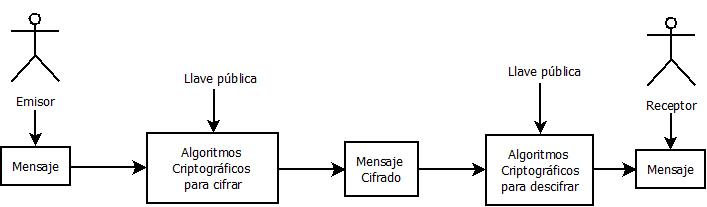
\includegraphics[width=10cm, height=5cm]{./images/sim.jpeg}
			\caption{Diagrama de criptografía simétrica.}
		\end{figure}
	\item La criptografía asimétrica: Utiliza una clave para el cifrado y otra para el descifrado, ver figura 1.2. [4]
		\begin{figure}[H]
			\centering
			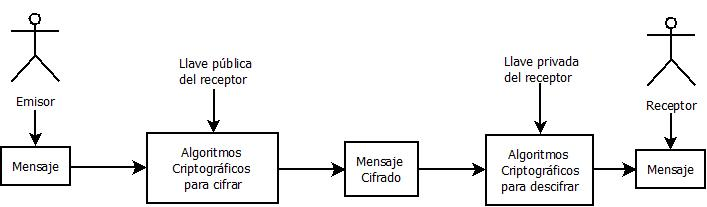
\includegraphics[width=10cm, height=5cm]{./images/asim.jpeg}
			\caption{Diagrama de criptografía asimétrica.}
		\end{figure}
\end{itemize}

Puesto que ambas cuestiones, la eliminación de duplicados y la privacidad de la información, son importantes, se ha comenzado a
proponer mecanismos que solucionen ambos problemas de manera conjunta, que son: Dupless ~\cite{Bellare}, ABS: the apportioned backup
system. ~\cite{abs}, Flud Backup ~\cite{flud}, SIGOPS Oper. Syst. ~\cite{sigops}, TahoeFS ~\cite{tahoe}.


\section{Justificación}

En la actualidad millones de personas usan los servicios de almacenamiento que ofrece la nube, ya sean gratuitos o privados, este número de personas ha ido en un incremento exponencial lo cual hace que el espacio de almacenamiento disminuya, entonces ¿Cómo podría mitigar el problema de almacenamiento y tener privacidad de los datos al mismo tiempo?

Usando la criptografía clásica para poder cifrar un archivo se utiliza una clave privada la cuál es distinta para cada usuario, cada vez que se cifra un archivo el resultado de este es diferente para cada intento. Por tanto no se puede evitar la duplicación de archivos utilizando este mecanismo de la criptografía y se deben implementar soluciones más robustas.

Una solución para tener privacidad y evitar duplicación la proporcionó John R. Douceur, la cual dice que teniendo a M que será el contenido de un archivo de aquí en adelante denominado el mensaje, el cliente primero calcula una clave K ← H(M) mediante la aplicación de una función de hash criptográfica H al mensaje y luego calcula el texto cifrado C ← E(K,M) a través de un esquema de cifrado simétrico determinista. El derivado del mensaje K se almacena por separado cifrándolo con una llave por cliente. Un segundo cliente B cifra el mismo archivo M que producirá el mismo C, evitando la duplicación. ~\cite{donceur}

En el artículo publicado por Mihir Bellare, Sriram Keelveedhi, Thomas Ristenpart, nombrado “DupLESS: Server-Aided Encryption for Deduplicated Storage” ~\cite{Bellare}, se observó que uno de los principales problemas al que nos enfrentamos es que el esquema de cifrado solo es seguro cuando el espacio de mensajes es demasiado grande, por lo tanto agentes externos pueden provocar agravios a la integridad de la información de los usuarios.

Si bien esta solución se ocupa de la duplicación de archivos deja muy vulnerable el aspecto de la privacidad, ya que ante un espacio de mensajes pequeño las amenazas del adversario son demasiadas. Si se tuvieran como ejemplo 1000 mensajes, para el adversario sería muy fácil intentar encontrar la clave, probando las 1000 claves posibles generadas con la función hash, hasta descifrar el archivo, por lo tanto se comprueba que un espacio de 1000 mensajes sigue siendo pequeño.

Es por ello que este trabajo terminal tiene como principal meta atacar esta problemática de privacidad, proponiendo una arquitectura del sistema que a través de un servidor de llaves se generaran llaves de acuerdo al contenido del archivo, para con esta se pueda cifrar y luego almacenar en la nube donde se eludirá la duplicación de archivos. Dicha arquitectura se explica con detalle en el siguiente apartado.

\section{Objetivos} % (fold)

Diseñar un sistema que evite la duplicación de archivos, garantizando la privacidad de los usuarios contra adversarios cuando el espacio de mensajes es pequeño, utilizando algoritmos criptográficos para su implementación.

    \subsection{Objetivos Generales} % (fold)
    
    
     
    \subsection{Objetivos Específicos} % (fold)
    
    
                
